\documentclass[10pt,a4paper,twoside,onecolumn]{book}
% Mes packages
\usepackage[utf8]{inputenc}
\usepackage[francais]{babel}
\usepackage[T1]{fontenc}
\usepackage{amsmath}
\usepackage{amsfonts}
\usepackage{amssymb}
\usepackage{graphicx}
\usepackage{lipsum} % Lorem Ipsum ...
\usepackage[Lenny]{fncychap} % Jolis en tête de chapitres
\usepackage{minitoc} % Mini table of contents
% COnfiguration des headers et footers
\usepackage{fancyhdr}
\fancyhead[CE]{} 
\fancyhead[LE]{}
\fancyhead[RE]{\rightmark}
\fancyhead[CO]{} 
\fancyhead[LO]{\leftmark}
\fancyhead[RO]{}
\fancyfoot[CO]{\thepage} 
\fancyfoot[LO]{}
\fancyfoot[RO]{}
\fancyfoot[CE]{\thepage} 
\fancyfoot[LE]{}
\fancyfoot[RE]{}
\pagestyle{fancy}
% Geometrie de la page
\usepackage[top=2cm, 
            bottom=2cm, 
            outer=1cm, 
            inner=2.1cm, 
            headsep=14pt]{geometry}
% Définitions diverses
\title{Ma thèse en une après-midi}
\author{Ludovic}

% Mes environnements
\newcommand{\epigraph}[2]
  {
  
  \og \textit{#1} \fg
  
  \textbf{#2}

  \vspace{1cm}

  \minitoc
  \newpage
  }

\begin{document}
\maketitle
\dominitoc% Initialization
\tableofcontents

\frontmatter %Préambule
% Le chapitre introduction de ma thèse
\chapter{Introduction}

\epigraph{S'il n'y a pas solution, c'est qu'il n'y a pas de problème}{Les Shadoks}

\lipsum[1-4]

\section{La limace de mer}

\lipsum[2-4]

\section{L'autre limace de mer}


\mainmatter % Corps du document
% Le chapitre introduction de ma thèse
\chapter{La Limace de mer}
\epigraph{S'il n'y a pas solution, c'est qu'il n'y a pas de problème}{Les Shadoks}

\section{Une partie}
\lipsum[1-2]

\section{La limace de mer}
\begin{figure}[h]
\begin{center}
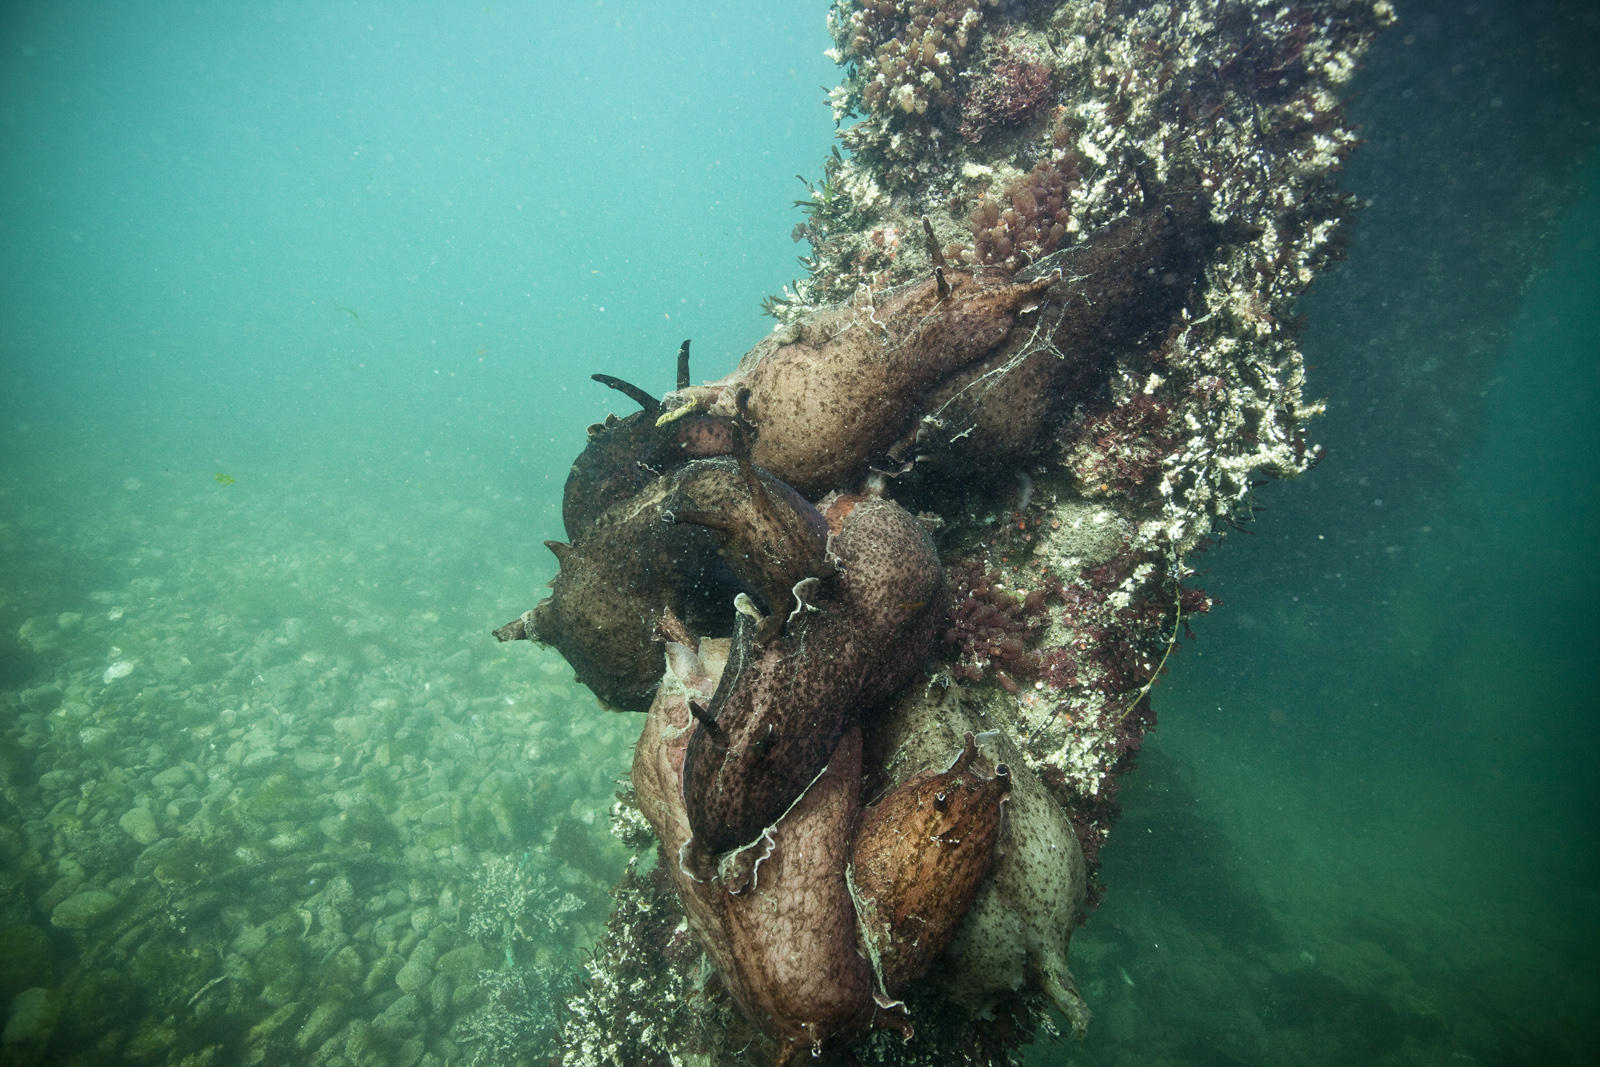
\includegraphics[width = .5\textwidth]{Chap1/figures/limace}
\end{center}
\caption{Un animal marin très intéressant}
\label{fig:limace}
\end{figure}

On observe la figure \ref{fig:limace} (page \pageref{fig:limace}) qui est très explicite\footnote{\href{https://fr.wikipedia.org/wiki/Aplysia}{Wikipedia}}. Un très bon article de Johnson \cite{Johnson, Zoran}, \citep[chapitre 3]{Johnson}.
\lipsum[1-2]

\section{L'autre limace de mer}
\lipsum[2-4]

\section{L'autre limace de mer}
\lipsum[2-5]
\backmatter % Annexes
\end{document}
